\documentclass[a4paper]{article}

\usepackage[utf8]{inputenc}
\usepackage[T1]{fontenc}
\usepackage[french]{babel}
\usepackage{fullpage}
\usepackage{hyperref}
\usepackage{amsmath}
\usepackage{amssymb}
\usepackage{upgreek}
\usepackage{color}
\usepackage[]{algorithm2e}
\usepackage{stmaryrd}
\usepackage{graphicx}
\usepackage{float}

\title{
    ELEC-H-201 - Electronique\\
    \small Synthèse 2014-2015
}
\author{Florentin \bsc{Hennecker}}
\date{}

\begin{document}
\maketitle
\tableofcontents

\section{Vademecum d'électricité (chapitre 2)}

    \subsection{Notions fondamentales}

    \subsubsection{Schémas}
    \begin{itemize}
        \item La \textit{charge} d'un montage est l'équipement/composant en aval d'un montage
        \item La \textit{source} d'un montage est l'équipement/composant en amont d'un montage
        \item Un montage est \text{à vide} si il n'y a pas de charge
        \item Un montage est \text{en charge} si il y a une charge
        \item Deux composants sont connectés en \textit{série} s'ils sont parcourus par le même courant
        \item Deux composants sont connectés en \textit{parallèle} s'ils sont soumis à la même ddp
        \item Un \textit{noeud} est une connexion entre plusieurs composants adjacents. La tension est la même à tout endroit du noeud (équipotentiel)
        \item Une \textit{maille} est une boucle fermée dans un schéma
        \item Une \textit{branche} est une suite de composants mis en série
    \end{itemize}

    \subsubsection{Courants et tensions}

    \paragraph{Intensité} L'\textit{intensité} ou le \textit{courant} 
    est le "débit" de charge électrique : $i() = \frac{dq(t)}{dt}$ en ampères. 
    (\textcolor{red}{[A] = [C/s]}) Elle se mesure avec un ampèremètre en série.
    Ses valeurs courantes vont de $10\mu$A à 100mA.\\

    Sur un schéma, les flèches représentent le \textit{courant conventionnel} formé
    de charges positives (dans le sens contraire du sens réel des électrons).

    \paragraph{Tension} La \textit{tension} est un terme flou et peut représenter 
    une force électromotrice, le potentiel d'un noeud ou la ddp aux bornes d'un dipôle.
    Elle se mesure en \textcolor{red}{[V] = [J/C]}) et oscillera dans ce cours entre 
    100$\mu$V à 100V.

    \paragraph{Potentiel} Le \textit{potentiel électrique} en un point vaut l'énergie
    à dépenser pour amener en ce point une charge électrique unitaire (1C) depuis
    un point où, par convention, ce potentiel vaut 0V.

    \paragraph{Masse} La masse est, par convention, le noeud qui vaut 0V. Attention, 
    masse $\neq$ terre! 

    \paragraph{Force électromotrice} La ddp d'une source idéale est appelée \textit{force électromotrice} (fig \ref{fig:fem})

    \begin{figure}[H]
        \begin{center}
            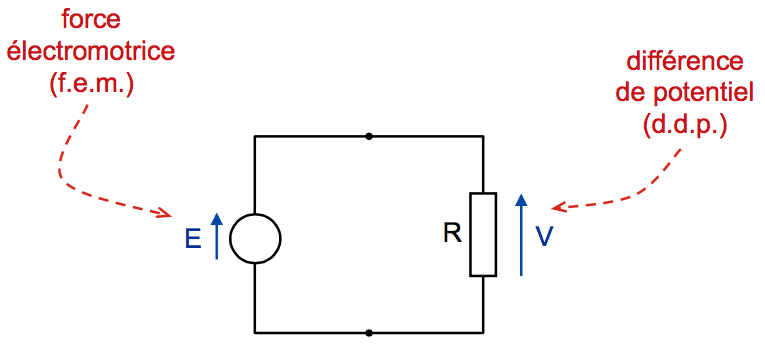
\includegraphics[width=0.6\textwidth]{fig/2_fem.png}
            \caption{Une force électromotrice}
            \label{fig:fem}
        \end{center}
    \end{figure}

    Convention de représentation de la ddp : la flèche de tension pointe vers le
    potentiel le plus positif.

    \subsubsection{Energie et puissance}

    \paragraph{Charge} La charge se mesure en \textcolor{red}{[C]}). Un électron
    porte une charge élémentaire négative notée $e$, qui vaut environ $-1,6.10^{-19}$C.

    \paragraph{Puissance} La puissance se mesure en \textcolor{red}{[W]}) et
    oscillera dans ce cours entre 10$\mu$W et 10W.

    \subsubsection{Energie et puissance}
    Formule de la puissance instantanée : $$ p(t) = v(t).i(t) $$

    \paragraph{Convention récepteur} Les flèches de courant et de tension sont
    de sens opposés

    \paragraph{Convention générateur} Les flèches de courant et de tension sont
    de même sens\\

    Dans les deux cas, $i>0$ et $v>0$.

    \paragraph{Dipôle passif} Un dipôle est \textit{passif} si il consomme de la puissance. On utilise alors la convention récepteur

    \paragraph{Dipôle actif} Un dipôle est \textit{actif} si il produit de la puissance. On utilise alors la convention générateur

    \subsubsection{Etat électrique, loi et caractéristique d'un dipôle}
    L'\textit{état électrique} d'un dipôle est le couple (I,V) de valeurs de
    courant et de tension qui s'appliquent à ce dipôle à un moment donné.

    \paragraph{Loi d'Ohm} $V = R.I$ (aussi appelée loi fondamentale d'un dipôle)

    \paragraph{Caractéristique} La \textit{caractéristique d'un dipôle} est le
    graphe représentant sa loi fondamentale dans le plan (I,V). Le point de fonctionnement
    du dipôle ne peut voyager que sur la caractéristique. \\
    \textbf{Exemple} : la caractéristique d'une source de tension idéale est une
    droite verticale (V constant).

    \paragraph{Résolution} On peut résoudre le circuit soit analytiquement, soit
    graphiquement (intersection des caractéristiques).

    \subsubsection{Principaux dipôles idéaux}
    \paragraph{Résistance} La résistance transforme la puissance électrique reçue
    en énergie thermique. Son unité est l'ohm \textcolor{red}{[$\Omega$]}, et
    oscillera dans ce cours entre $10\Omega$ et $10M\Omega$
    \begin{figure}[H]
        \begin{center}
            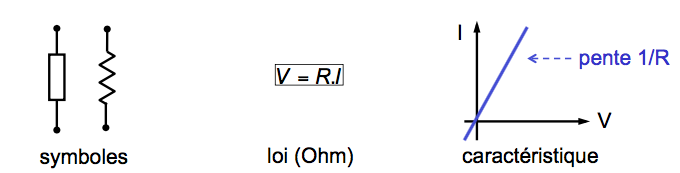
\includegraphics[width=0.6\textwidth]{fig/2_resistance.png}
            \caption{Dipôle résistance}
        \end{center}
    \end{figure}

    \paragraph{Source de tension} Ce dipôle fixe la tension.
    \begin{figure}[H]
        \begin{center}
            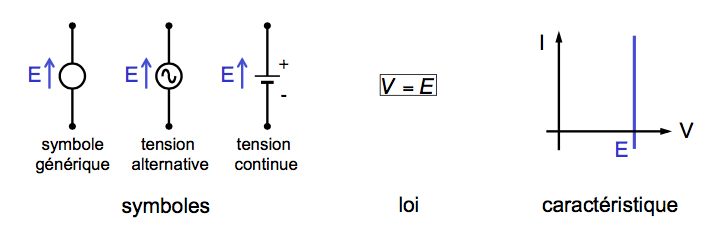
\includegraphics[width=0.6\textwidth]{fig/2_sourcetension.png}
            \caption{Source de tension}
        \end{center}
    \end{figure}

    \paragraph{Source de courant} Ce dipôle fixe le courant.
    \begin{figure}[H]
        \begin{center}
            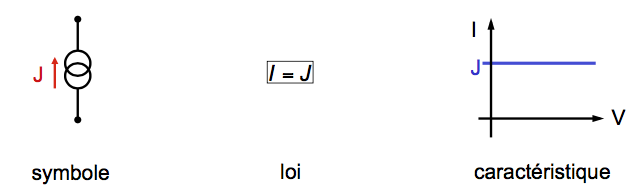
\includegraphics[width=0.6\textwidth]{fig/2_sourcecourant.png}
            \caption{Source de courant}
        \end{center}
    \end{figure}

    \paragraph{Court-circuit} Dipôle dans lequel la tension est nulle.
    \begin{figure}[H]
        \begin{center}
            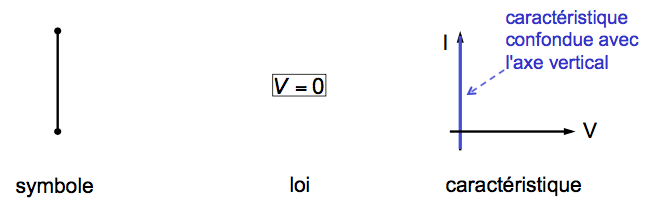
\includegraphics[width=0.6\textwidth]{fig/2_courtcircuit.png}
            \caption{Court-circuit}
        \end{center}
    \end{figure}

    \paragraph{Circuit ouvert} Dipôle dans lequel le courant est nul.
    \begin{figure}[H]
        \begin{center}
            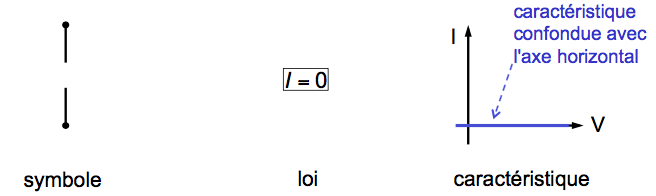
\includegraphics[width=0.6\textwidth]{fig/2_circuitouvert.png}
            \caption{Circuit ouvert}
        \end{center}
    \end{figure}

    \paragraph{Capacité} Sa caractéristique n'est pas représentable sur (I,V) car
    elle fait intervenir la notion de temps. Une capacité s'exprime en farads
    \textcolor{red}{[F]} et oscillera entre 10pF et 1mF.
    \begin{figure}[H]
        \begin{center}
            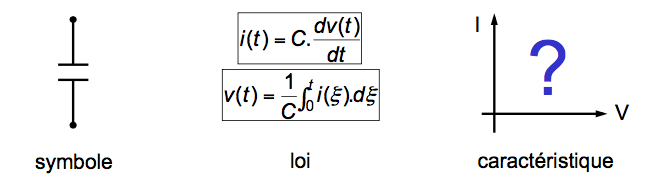
\includegraphics[width=0.6\textwidth]{fig/2_capacite.png}
            \caption{Capacité}
        \end{center}
    \end{figure}

    \paragraph{Inductance} Sa caractéristique n'est pas représentable sur (I,V) non plus.
    Les self-inductances sont exprimées en henris \textcolor{red}{[H]} et oscillent
    entre 10nH et 100mH.
    \begin{figure}[H]
        \begin{center}
            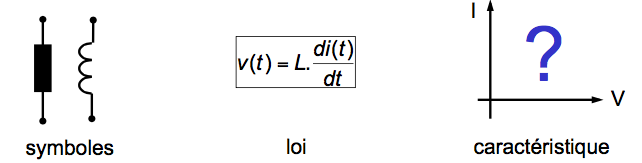
\includegraphics[width=0.6\textwidth]{fig/2_inductance.png}
            \caption{Capacité}
        \end{center}
    \end{figure}

    La capacité et l'inductance ont un statut particulier : elles ne dissipent
    pas de puissance mais sont capables d'emmagasiner de l'énergie et de la 
    restituer ensuite. Ces dipôles sont \textit{réactifs}.\\

    \'A un instant donné, l'énergie accumulée par ces composants vaut : 
    $E = \frac{C.V^2}{2}$ ou $E = \frac{L.I^2}{2}$\\

    \paragraph{Linéarité} On dit qu'un dipôle est \textit{linéaire} si sa caractéristique est une droite. Les systèmes linéaires bénéficient de propriétés particulières utiles. Les capacités et inductances sont considérées linéaires car elles peuvent s'exprimer linéairement en terme de charge électrique.
    $Q=C*V$
    $\phi=L*I$

\section{Amplificateurs opérationnels (Chapitre 4)}
    \subsection{Pourquoi amplifier}
        \begin{itemize}
            \item Signaux très faibles
            \item Régler le niveau logique
            \item Amplifier en amont d'un CAN/ADC (Convertisseur Analogique/Numérique)
        \end{itemize}

    \subsection{Propriétés de base}
        \subsubsection{Définitions}
            \begin{figure}[H]
                \begin{center}
                    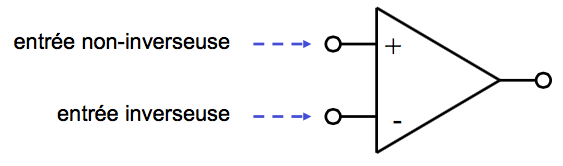
\includegraphics[width=0.6\textwidth]{fig/4_ampliop.png}
                    \caption{Ampli Op}
                \end{center}
            \end{figure}
            \begin{itemize} 
            \item C'est un circuit intégré à 8 pattes (deux bornes d'entrée et une borne de sortie). Il est considéré comme un quadripôle.
            \item L'entrée $-$ est l'entrée \textit{inverseuse}.
            \item L'entrée $+$ est l'entrée \textit{non-inverseuse}.
            \item Chacune des entrées et sortie reçoit un signal de tension mesuré par rapport à la masse. Ils sont notés respectivement $ V^{+} $, $ V^{-} $ et $ V_{out} $
            \item La \textit{tension d'entrée différentielle} est notée $ V_{d} = V^{+} - V^{-} $
            \item La fonction d'un ampli-op est d'amplifier cette tension
            \end{itemize}
        \subsubsection{Loi fondamentale et gain}
        La \textit{fonction d'amplification} d'un ampli-op est $ V_{out} = A*V_{d} $ \\
        Le \textit{gain} $A$ d'un ampli op est le facteur d'amplification entrée son entrée différentielle et sa sortie. \\
        \begin{itemize}
            \item $A$ est sans dimension.
            \item $A$ est très élevé (typiquement entre 30000 et 100000). On fait l'hypothèse qu'il est infini.
            \item $A$ n'a de sens que si la tension d'entrée est très faible.
            \item Les tensions $V_{d}$ et $V_{out}$ peuvent être aussi bien positives que négatives (par exemple dans le cas d'un courant alternatif)
        \end{itemize}

        \subsubsection{Bornes d'alimentation}
            \begin{figure}[H]
                \begin{center}
                    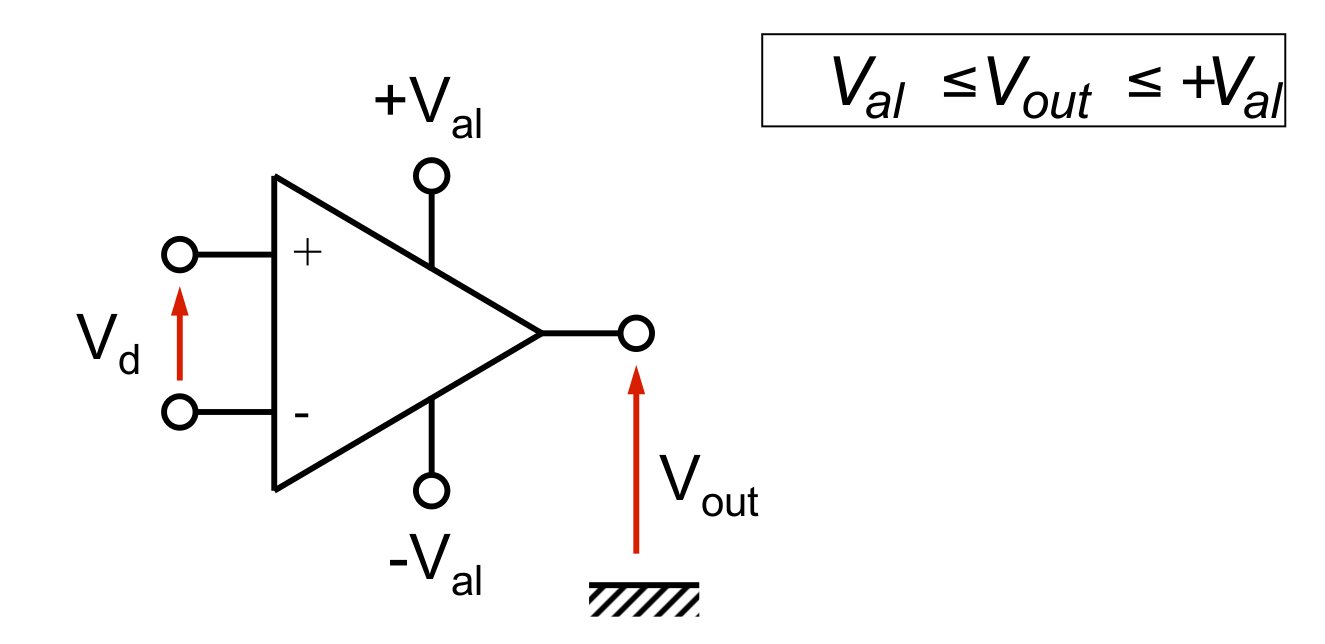
\includegraphics[width=0.6\textwidth]{fig/4_ampliop_alim.png}
                    \caption{Ampli Op}
                \end{center}
            \end{figure}
            Pour amplifier le signal, l'ampli-op a besoin d'une source d'énergie qui est fournie par des bornes d'alimentation.\\
            \begin{itemize}
                \item Elles sont le plus souvent symétriques
                \item Généralement $-12V$ et $+12V$ ou $-15V$ et $+15V$
                \item La tension de sortie ne peut pas sortir de la gamme fixée par ces tensions d'alimentation
            \end{itemize}
            L'ampli op est donc un composant \textbf{actif} car il ajoute de la puissance dans le circuit.
    \subsection{Ampli-Op réel : 741}
        \begin{figure}[H]
            \begin{center}
                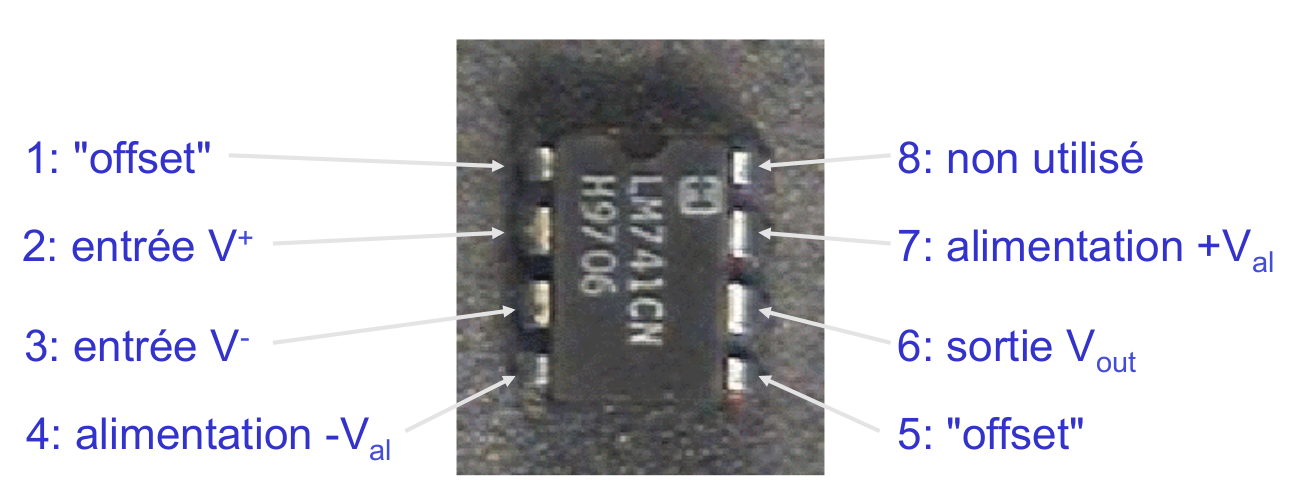
\includegraphics[width=0.6\textwidth]{fig/4_ampliop_reel.png}
                \caption{Ampli Op}
            \end{center}
        \end{figure}


\end{document}